\documentclass{article}
\usepackage{graphics, graphicx}
\usepackage[UTF8]{ctex}
\usepackage{geometry}
\usepackage{amsmath}
\geometry{
    a4paper, 
    total={170mm, 257mm}, 
    top=20mm, 
    left=20mm, 
}

\begin{document}
\begin{center}
    Mean Shift 算法
\end{center}
\begin{center}
\begin{tabular}{c c c c c}
    \hline
    \hline
    学院 & 年级 & 班级 & 姓名 & 学号 \\
    \hline
    控制科学与工程 & 2017级 & 人工智能与机器人 & 陈逸群 & 201700181055 \\
    \hline
    \hline
\end{tabular}
\end{center}
\tableofcontents
\newpage
\section{简介}
Mean Shift是一个理解容易实现简单的聚类算法,具有通用、非参数化、与聚类形状无关的特点,
最早由Fukunage在1975年被提出,但最初并没有得到足够的重视。1995年Yizong Cheng定义了一族核函数,
使得各样本点对被偏移点的Mean Shift向量的贡献随着距离的变化而变化;其次,作者还定义了权重系数,使得不同样本
点的重要性不尽相同,扩大了Mean Shift算法的应用范围。

\section{基本思想}
Mean Shift是基于KDE(Kernel Density Estimation)的算法,给定一个由n个维度为d的独立同分布的样本组成的数据集
$ \{x_1, x_2, \ldots, x_n\} $,现在想要估计这些样本的概率分布,在d维空间中的每一个样本处放置一个核函数,
由于核函数表示的是以该样本点为中心的权重分布,不同样本点会得到不同的权重,将所有样本点的权重相叠加,
那么在整个空间中就会形成一个概率分布,选择核函数的不同的带宽h会导致不同的概率分布。将局部极大值视为样本点
的不同类别,那么将这些样本点归到极大值所对应的类别中就完成了聚类。该聚类过程不需要显式指定类别数,而是调整
带宽h。由于带宽h控制核函数的概率分布的形状,进而控制所有样本点形成的概率分布,也相当于间接控制了类别数。

下图表示在每一个样本点放置一个核函数所形成的概率密度分布,图中共有三个极大值,每个极大值对应一个类别,
那么就可以将每一个样本点分配到相应的极大值对应的类别中,这便是Mean Shift算法所要做的。

\begin{center}
    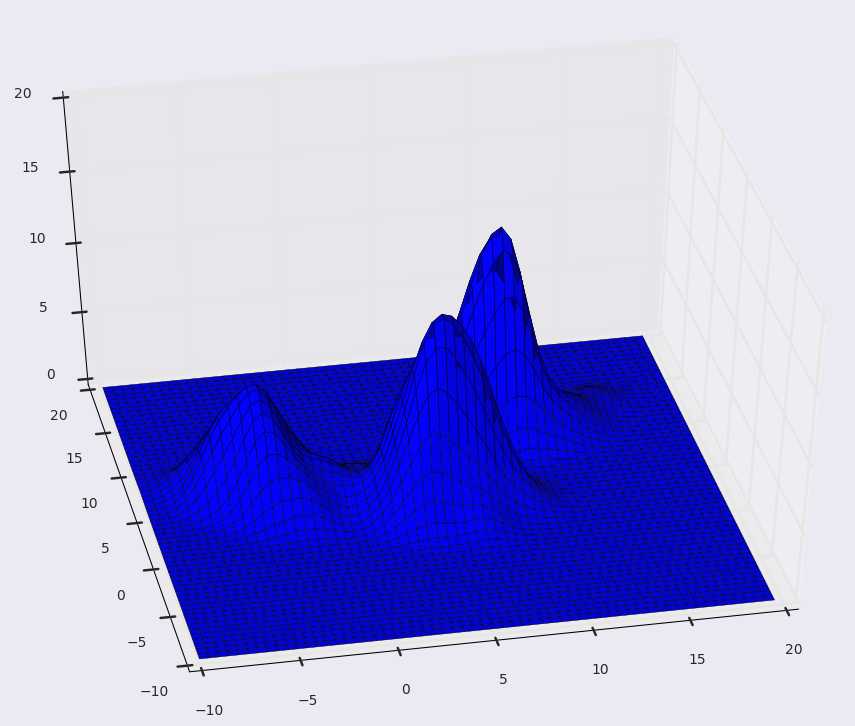
\includegraphics[width=0.7\textwidth]{Images/example_kde_2.png} \\

    图1 KDE
\end{center}

对于拟合的概率密度分布,其极大值表示该位置更有可能生成样本点,亦即大部分生成的样本都集中在此,呈现“聚集”
特点,因而可以将该极大值及其附近的样本点聚为一类。

Mean Shift算法将确定每一个样本点的所属极大值范围,其基本依据是概率分布的梯度。对于每一个样本点,沿着其梯度
的反方向一直行进,最终可以到大某一个极大值点,该极大值点所对应的类别便作为该样本点的类别。因此,该算法的
一个重点就是找到梯度的反方向。我们假设某个极大值点为某一个类的中心(质心),而某一范围的质心便是该范围
的所有样本点的位置的均值(假设每一个样本对形成质心的贡献均一致),因此,对于某一个样本点而言,选定一个区域,
该样本点到该区域的质心的向量便可以近似表示为该样本点到其对应的极大值点的梯度的反方向,以该样本点为起点,
以该区域的质心为终点所确定的向量便称为Mean Shift向量。

\begin{center}
    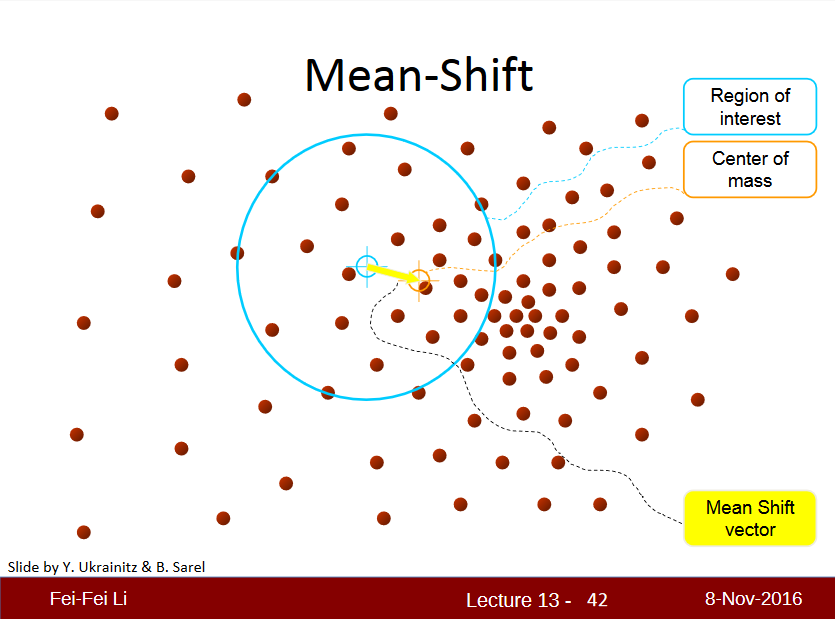
\includegraphics[width=\textwidth]{Images/MeanShift1.png}
    图2 Mean Shift向量
\end{center}

\section{Mean Shift算法原理}
\subsection{Kernel Density Estimation}
Kernel Density Estimation简称KDE,是一种用来估计概率密度函数的非参数方法,可以看成是由一系列核函数拟合
所需要的概率密度函数。给定一个由n个独立同分布的样本组成的数据集$ \{x_1, x_2, \ldots, x_n\} $,假设其
概率密度函数为f,那么可以利用核函数来拟合概率密度函数f:
\begin{align}
    \hat{f_h}(x) &= \frac{1}{n} {\sum}_{i=1}^nK_H(x_i - x) \\
    K_H &= |H|^{-\frac{1}{2}} K(H^{-\frac{1}{2}} x) 
\end{align}
其中,H是一个d维正定对称的带宽(Bandwidth)矩阵,通常取$ H = diag\{h_1^2, h_2^2, \ldots, h_d^2\} $
或者$ H = h^2I $, $h$为带宽bandwidth,是可调参数,$K(\cdot)$ 为d维核函数,满足以下性质:
\begin{itemize}
    \item $K(\cdot) \ge 0$
    \item $ {\int}_{{\Re}^d} K(\cdot)dx = 1 $
    \item $ {lim}_{||x|| \rightarrow \infty} ||x||^dK(x) = 0$
    \item 数学期望(均值)为0:$ {\int}_{{\Re}^d} xK(x)dx = 0 $
    \item $ {\int}_{{\Re}^d} xx^TK(x)dx = C_K I $
\end{itemize}
d维核函数K(x)可以从一个对称单变量核函数$K_1(x)$通过两种形式生成:
\begin{align}
    K^p(x) &= {\prod}_{i=1}^d K_1(x_i)\\
    K^s(x) &= a_{k, d}K_1(||x||)
\end{align}
其中$K^s(x)$为径向对称核函数,通常会更合适,在Mean Shift中将用它构建算法。

Mean Shift采用$K(x) = c_{k, d}k(||x||^2)$的形式,其中系数$c_{k, d}$为归一化系数,使K(x)满足以上核函数的性质。

通常采用的核函数有两种,一种使高斯核函数,另一种为Epanechnikov核函数。对于高斯核函数,有
\begin{align}
    k_N(x) &= e^{-\frac{1}{2}x} \\
    K_N(x) &= \frac{1}{{\sqrt{2\pi}}^d} e^{-\frac{1}{2}||x||^2}
\end{align}
对于Epanechnikov核函数,有
\begin{align}
    k_E(x) &= \begin{cases}
        1-x, 0 \leq x \leq 1 \\
        0, otherwise \\
    \end{cases} \\
    K_E(x) &= \begin{cases}
        \frac{1}{2} C_d^{-1}(d+2)(1-||x||^2) \\
        0, otherwise \\
    \end{cases}
\end{align}

根据以上理论,可以将概率密度估计为
\begin{align}
    \hat{f_{h, k}} (x) &= \frac{1}{n} {\sum}_{i=1}^nK_H(x-x_i) \\
    &= \frac{1}{n} {\sum}_{i=1}^n |H|^{-\frac{1}{2}} K(H^{-\frac{1}{2}}(x-x_i)) \\
    &= \frac{1}{nh^d} {\sum}_{i=1}^n K(\frac{x-x_i}{h}) \\
    &= \frac{c_{k, d}}{nh^d} {\sum}_{i=1}^n k(||\frac{x-x_i}{h}||^2) 
\end{align}

我们要寻找的模式位于概率密度最大的地方,也就是梯度为0的地方:$ \nabla f(x) = 0 $,
我们以f(x)的梯度估计值来代替f(x)的梯度,即$ \nabla f(x) = \hat{\nabla} f(x) $。由于f(x)不能直接得到,
因此我们采用f(x)的估计值的梯度来代替f(x)梯度的估计值,即:$ \nabla \hat{f_{h, k}}(x) = \hat{\nabla} f_{h, k}(x) $
即:
\begin{align}
    \hat{f}_{h, k}(x) &= \frac{c_{k, d}}{nh^d}{\sum}_{i=1}^n k(||\frac{x-x_i}{h}||^2) \\
    \nabla f_{h, k}(x) &= \nabla \hat{f}_{h, k}(x) \\
    &= \frac{2c_{k, d}}{nh^{d+2}} {\sum}_{i=1}^n k'(||\frac{x-x_i}{h}||^2)(x-x_i) 
\end{align}

我们定义另一个核函数$ G(x) = c_{g, d}g(||x||^2) = - c_{g, d} k'(||x||^2) $,那么我们可以得到概率密度梯度
估计值为:
\begin{align}
    \hat{\nabla} f_{h, k}(x) &= \nabla \hat{f}_{h, k}(x) \\
    &= \frac{2c_{k, d}}{nh^{d+2}} {\sum}_{i=1}^n (x_i-x)g(||\frac{x-x_i}{h}||^2) \\
    &= \frac{2c_{k, d}}{nh^{d+2}} [{\sum}_{i=1}^n x_i g(||\frac{x-x_i}{h}||^2) - x{\sum}_{i=1}^n g(||\frac{x-x_i}{h}||^2)] \\
    &= \{\frac{2c_{k, d}}{nh^{d+2}}[{\sum}_{i=1}^ng(||\frac{x-x_i}{h}||^2)]\}\{\frac{{\sum}_{i=1}^nx_ig(||\frac{x-x_i}{h}||^2)}{{\sum}_{i=1}^ng(||\frac{x-x_i}{h}||^2)} - x\}
\end{align}
其中,第一项与另一个核函数的密度估计值有关,记为
\begin{equation}
    \hat{f}_{h, G}(x) = \frac{c_{G, d}}{nh^d} {\sum}_{i=1}^n g(||\frac{x-x_i}{h}||^2)
\end{equation}
第二项便是mean shift向量,记为
$$ 
m_{h, G}(x) = \frac{{\sum}_{i=1}^nx_ig(||\frac{x-x_i}{h}||^2)}{{\sum}_{i=1}^ng(||\frac{x-x_i}{h}||^2)} - x
$$
因此,
$$
\nabla \hat{f}_{h, K}(x) = \frac{2c_{k, d}}{h^2c_{g, d}} \hat{f}_{h, G}(x) m_{h, G}(x)
$$
那么可以得到mean shift向量:
$$
m_{h, G} = \frac{1}{2} \frac{c_{g, d}}{c_{k, d}} h^2 \frac{1}{\hat{f}_{h, G}(x)} \nabla \hat{f}_{h, K}(x)
$$
由于$ \hat{f}_{h, G}(x) $其实是一个标量,所以我们可以知道mean shift向量与梯度方向成比例,且mean shift方向
指向概率密度增加最快的方向。越靠近极大值点,mean shift向量的模越小,因此这是一个自适应的梯度上升方法,它与
其他梯度上升的方法相比,具有不需要选择合适的步长的优点。

\subsection{基本算法}
给定一个数据集,该算法的最终目标为在给定核函数的情况下,将每一个样本点沿着核函数确定的概率分布的梯度反方向
移动到某一个局部极大值处,以确定该样本点的所属类别。\\

\begin{center}
\begin{tabular}{l}
    \hline 
    \hline
    \textbf{Input}: Dataset {$ \{x_1, x_2, \ldots, x_n\}, x_i \in {\Re}^d $}, Bandwidth $h$\\
    Copy all samples into a new space. \\
    In the new space, \\
    \textbf{for} $ x_i \in \{x_1, x_2, \ldots, x_n \} $\\
    \quad \quad \textbf{do}: \\
    \quad \quad \quad \quad $ S_k(x_i) = \{y: (y-x_i)^T(y-x_i) \le h^2 \} $ \\
    \quad \quad \quad \quad $ M_h(x_i) = \frac{1}{K} {\sum}_{x_j \in S_k} (x_j - x) $ \\
    \quad \quad \quad \quad $ x_i = x_i + M_h(x_i) $ \\
    \quad \quad \textbf{while} $ M_h(x_i) < \epsilon $ \\
    \quad \quad Record the center with a radius. \\
    \textbf{end} \\
    Label every cener a class. \\
    \textbf{Output}: every sample with a class label. \\
    \hline 
    \hline
\end{tabular}

Mean Shift的基本算法
\end{center}

通过该算法,每一个样本点都要经过移动直至收敛,那么收敛点及到达其附近某一邻域的所有样本点都归为同一类。
该算法的时间复杂度为$ O(n^2) $,显然计算量太大,对该算法可以进行三方面的改进:
\begin{itemize}
    \item 某一个样本点收敛后,其以r为半径的超球域内的所有点不必再计算,直接归为同一类;
    \item 某一个样本点在搜索的时候,以c为半径的超球域内的点不再计算,直接归为同一类;
\end{itemize}
\subsection{优缺点}
Mean Shift的优点为:
\begin{itemize}
    \item Mean Shift算法为通用算法;
    \item 模型无关的算法,不需要对所需聚类的形状进行任何假设(如,球形,椭圆形等);
    \item 只需要调整超参数h;
    \item 对离群值的鲁棒性强;
\end{itemize}
Mean Shift的缺点为:
\begin{itemize}
    \item 输出取决于窗口大小h;
    \item 窗口大小h的选取并非唯一;
    \item 计算复杂度高;
    \item 对特征空间的维度放缩不够好;
\end{itemize}

\subsection{对Mean Shift的改进}
在Mean Shift的基本算法中,同一个球域内的所有点对Mean Shift向量的贡献是一样的,然而事实上并非如此,因此
对Mean Shift算法进行改进,将Mean Shift向量重新定义为:
$$ 
m_{h, G}(x) = \frac{{\sum}_{i=1}^nx_ig(||\frac{x-x_i}{h}||^2)}{{\sum}_{i=1}^ng(||\frac{x-x_i}{h}||^2)} - x
$$

\subsection{带宽的选择}
带宽的选择通常是经验性的,但是仍然有4个原则可供参考:
\begin{itemize}
    \item 最优带宽应该能够达到偏置和方差的最优折中,能够最小化误差;
    \item 带宽与稳定性有关,它被视为最大操作范围的中心,在该范围内,给定数据可以获得相同数量的簇;
    \item 最优带宽会最大化目标函数,该目标函数能表示结果的质量,通常比较类内的相似性与类间的多样性;
    \item 通常自顶向下的用户先验信息或者高层模块可以用来控制带宽。
\end{itemize}

\section{Mean Shift的应用简述}

\subsection{聚类}
由以上的分析过程,易知Mean Shift算法明显可以应用于样本点的聚类问题,聚类案例如下:
\begin{center}
    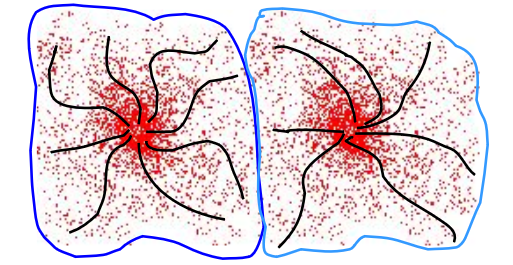
\includegraphics[width=\textwidth]{Images/cluster1.png}
    Mean Shift的应用:聚类
\end{center}

\subsection{图像分割}
图像分割的本质其实是聚类,图像的每一个像素都具有位置属性以及像素属性,其中像素属性描述颜色或者亮度等特征。
实际应用时,会对位置属性以及像素属性分配不同的权重。
\begin{center}
    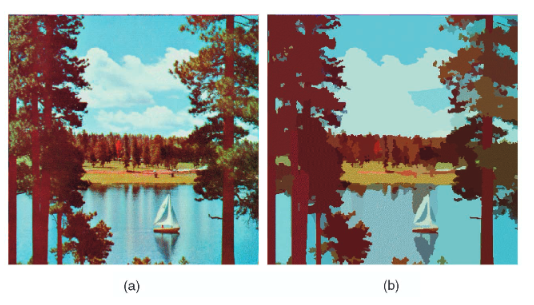
\includegraphics[width=\textwidth]{Images/segmentation1.png}
    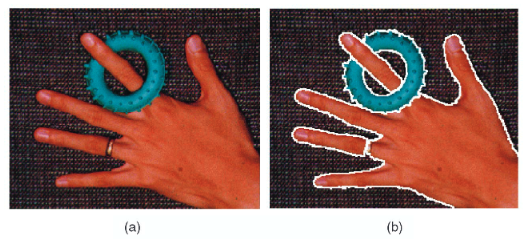
\includegraphics[width=\textwidth]{Images/segmentation2.png}
    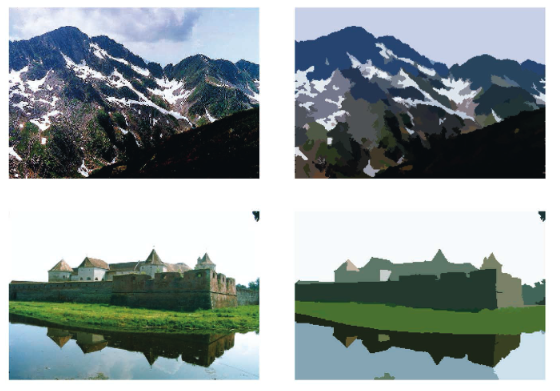
\includegraphics[width=\textwidth]{Images/segmentation3.png}
    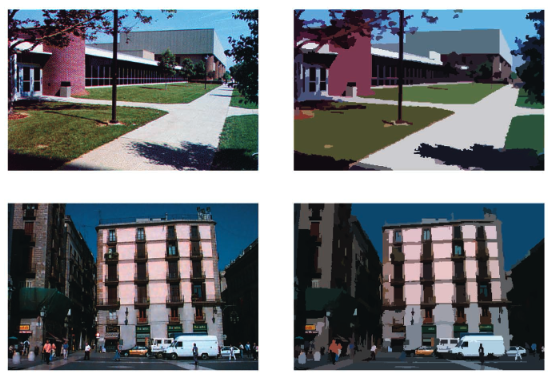
\includegraphics[width=\textwidth]{Images/segmentation4.png}

    Mean Shift的应用:图像分割
\end{center}

\subsection{图像平滑}
图像平滑与图像分割大同小异,图像平滑是一个去除高频信号保留低频信号的过程,它与图像分割的不同之处在于:
\begin{itemize}
    \item Mean Shift迭代的过程中,通常只迭代一次;
    \item 找到目标点之后,直接用目标点的颜色特征代替该点的颜色特征;
\end{itemize}
事实上,图像分割也可以视为图像平滑的结果。
\begin{center}
    
\includegraphics[width=\textwidth]{Images/smooth.png}

    Mean Shift的应用:图像平滑
\end{center}

\subsection{轮廓提取}
轮廓提取首先利用Mean Shift进行图像分割,然后根据分割结果,取不同区域的边界,便得到所需要的轮廓。
\begin{center}
    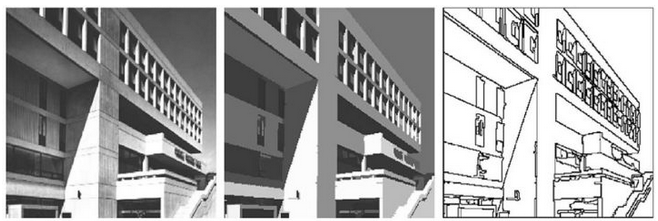
\includegraphics[width=\textwidth]{Images/profile.png}

    Mean Shift的应用:轮廓提取
\end{center}


\subsection{目标跟踪}
使用Mean Shift进行目标跟踪通常先对目标区域进行建模,一般而言对目标区域进行灰度颜色空间的均匀划分,
然后表示成灰度直方图,根据该灰度直方图建立目标模型的概率密度,然后进行候选区域表示,通常用同样的方法,
得到候选模型的概率密度,最后选择相似性度量函数衡量候选区域与目标区域的相似性程度,通常将前一帧中目标
的中心位置作为本帧搜索窗口的中心,寻找使得相似函数最大的候选区域,即确定本帧中目标的位置。
\begin{center}
    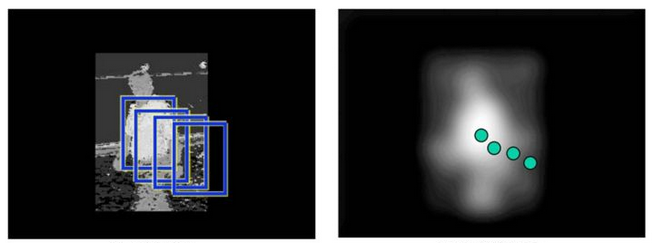
\includegraphics[width=\textwidth]{Images/tracking.png}

    Mean Shift的应用:目标跟踪
\end{center}

\section{参考资料}
[1] https://spin.atomicobject.com/2015/05/26/mean-shift-clustering/ 

[2] http://vision.stanford.edu/teaching/cs131\_fall1617/
lectures/lecture13\_kmeans\_mean\_shift\_cs131\_2016 

[3] Comaniciu, D., \& Meer, P. (2002). Mean shift: A robust 
approach toward feature space analysis. IEEE Transactions on 
Pattern Analysis and Machine Intelligence, 24(5), 603–619. https://doi.org/10.1109/34.1000236 
\end{document}